\section*{druhá mechanická varianta}
\addcontentsline{toc}{section}{druhá mechanická varianta}

Druhá mechanická varianta je až na drobnosti stejná jako verze dnešní.
Ovládá se pěti koly, z nichž čtyři zajišťují heslo a páté otáčí s rotační západkou, které drží dveře na svém místě.
Tato varianta tedy přichází z možností dveře úplně oddělit od skříně trezoru. To by při využití jako trezor, který
má za úkol jen ochraňovat svůj obsah, sice nepřinášelo žádný velký užitek, ale při mém využití, spíše jako herní 
prvek než trezor, to může být užitečné.

\begin{figure}[htbp]
    \centering
    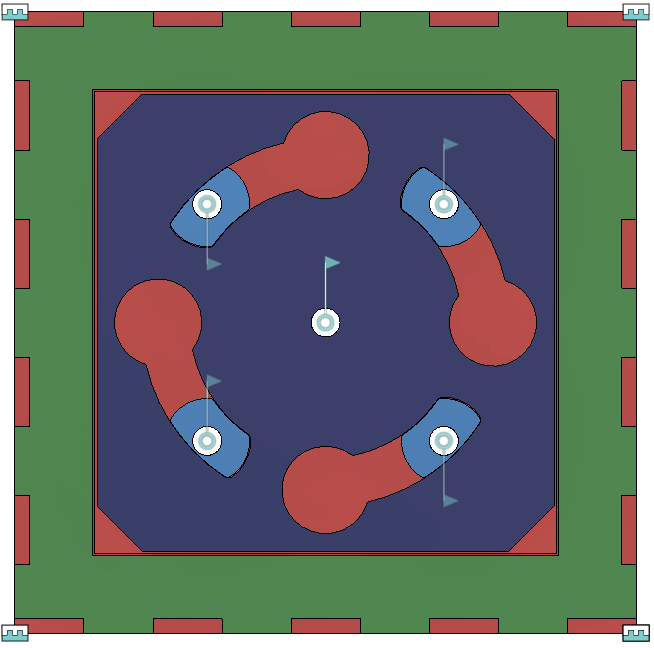
\includegraphics[width=150]{kapitoly/obrazky/M2-mechanizmus.png}
    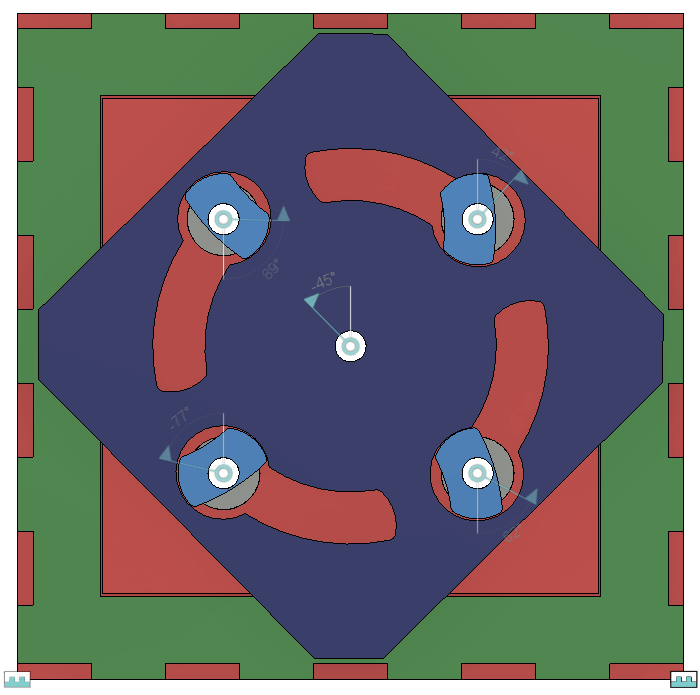
\includegraphics[width=150]{kapitoly/obrazky/M2-mechanizmus_zamceno.png}
    \label{fig:M1}
\end{figure}

\begin{figure}[htbp]
    \centering
    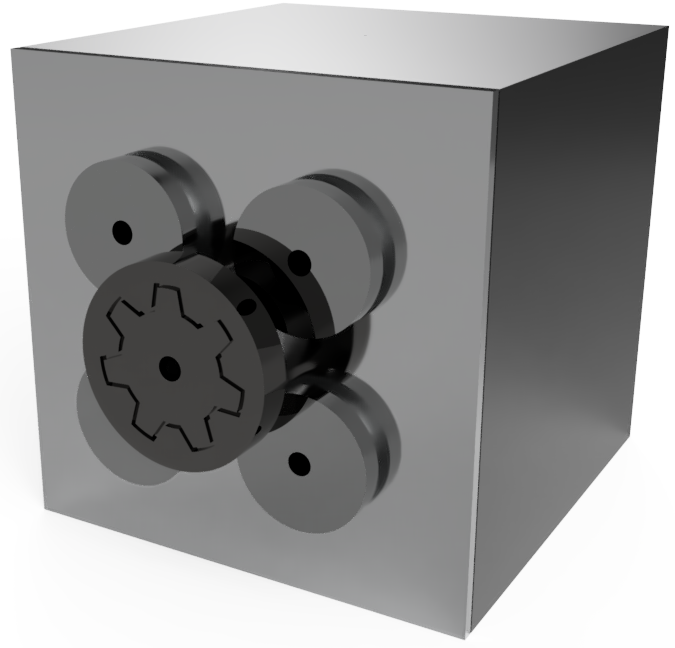
\includegraphics[width=\textwidth]{kapitoly/obrazky/M2-render.PNG}
    %\caption{}
    \label{fig:M1.0}
\end{figure}


\newpage